\section{Interpolation}

Digital delay lines are implemented using a memory buffer of discrete audio samples. To change the delay time, we change the distance in the buffer between where samples are written and where they are read back.\cite{reiss2014audio}
<<<<<<< HEAD
It is often necessary for a delay line to vary in length. Usually, separate read and write pointers are used. Additionally, for good quality audio, it is necessary to interpolate the delay-line length rather than ``jumping'' between integer numbers of samples. This is typically accomplished using an interpolating read to make the delay line vary smoothly over time.~\cite{smith2010physical}
In our work we tried implementing both linear interpolation and 2ndorder polynomial interpolation and the second one seemed to be the smoother one.

\paragraph{Linear Interpolation}
Linear interpolation is the most commonly used case because it is easy to implement and inexpensive.
It works by effectively drawing a straight line between two neighboring samples and returning the appropriate point along that line (see ~\ref{fig:linear-interpolation}).
=======
Separate read and write pointers are used and additionally, for good quality audio, it is necessary to interpolate the delay-line length rather than ``jumping'' between integer numbers of samples. This is typically accomplished using an interpolating read to make the delay line vary smoothly over time.~\cite{smith2010physical}
Since the delay of the flanger changes by small amounts each sample, it will inevitably take fractional values, so interpolation is always used when calculating the delayed signal of the flanger.

In our work we tried implementing both linear interpolation and polynomial interpolation and the second one seemed to be the smoother one.
We implemented them by writing the member function \texttt{interpolate} in the \texttt{PluginProcessor.cpp} file.


\paragraph{Linear Interpolation}
Linear interpolation is the most commonly used case because it is easy to implement and inexpensive.
It works by effectively drawing a straight line between two neighboring samples and returning the appropriate point along that line (see figure ~\ref{fig:linear-interpolation}).
>>>>>>> cfab2398a6d75feefbcce0876efa97dd25e02379
  
\begin{figure}[h]
	\centering
  	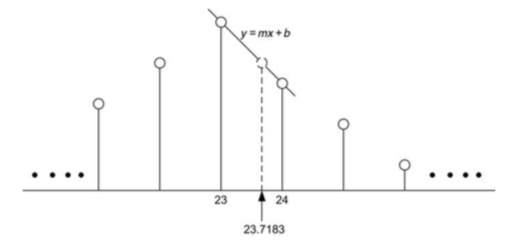
\includegraphics[width=0.8\linewidth]{assets/Linear interpolation of sample values.png}
  	\caption{Linear interpolation of sample values}
  	\label{fig:linear-interpolation}
\end{figure}

<<<<<<< HEAD


\paragraph{Polynomial Interpolation}
In polynomial interpolation a curve is drawn between the points (or a series of points), and then the interpolated value is found on that curve.~\cite{pirkle2013designing}
=======
This is given in the following equation:
\[
 x(t) = (n + 1 - t)x[n] + (t-n)x[n+1], 				n \leq t< n + 1
\]
where $x[n]$ and $x[n+1]$ are two successive  samples and $ (t-n) $ is a fractional value which is the difference between the reader pointer and the largest integer that is not grater than the reader pointer.

\paragraph{Polynomial Interpolation}
In a polynomial interpolation the function is estimated to be an Nth-order polynomial. A curve is drawn between the points (or a series of points), and then the interpolated value is found on that curve.~\cite{pirkle2013designing}

\[
 x(t) = c_{N}t^{N} + c_{N–1}t^{N–1} + ... c_{1}t^{1} + c_{0}, 				n \leq t< n + 1
 \]

Second-order polynomial interpolation considers three successive samples surrounding the interpolated location: $x[n-1]$, $x[n]$, and $x[n+1]$. 

\[
x(t) = c_{2}(t-n)^{2} + c_{1}(t-n) + c_{0}
\]

\[
c_{0} = x[n]
\]
\[
c_{1} = (x[n+1] - x[n-1])/2
\]
\[
c_{2} = (x[n+1] - 2x[n] + x[n-1])/2
\]
>>>>>>> cfab2398a6d75feefbcce0876efa97dd25e02379



